\documentclass{ximera}

\addPrintStyle{..}

\begin{document}
	\author{Bart Lambregs}
	\xmtitle{De derde wet van Newton}{}
    \xmsource\xmuitleg

Krachten komen niet uit het niets, ze worden altijd door een ander voorwerp uitgeoefend. Zo is het de hamer die de spijker in de muur drijft en is het de voet die een trap tegen de bal geeft. In deze voorbeelden oefent het ene voorwerp een kracht uit en ondergaat het andere voorwerp die kracht. Maar, is het zo eenzijdig \ldots? Het volgende voorbeeld geeft aan van niet. Het geeft aan dat er naast een `actie'kracht ook altijd een `reactie'kracht optreedt.

Meestal plooien vingers naar de handpalm toe. De praktijk leert dat het andersom toch iets moeilijker gaat, misschien vandaar. Als de andere hand echter wat helpt door te duwen (dus een kracht uitoefent op de vingers), plooien de vingers al iets verder naar achter; uit zichzelf geraken ze niet zo ver. Als je nu -- ter vergelijking -- met gestrekte vingers tegen de tafel duwt, plooien je vingers eveneens meer naar achteren dan dat ze uit zichzelf zouden kunnen. Omdat de vingers zonder een extern uitgeoefende kracht niet zo ver kunnen doorbuigen, valt te concluderen dat naast de kracht die door de vingers op de tafel wordt uitgeoefend, de tafel op zijn beurt een kracht uitoefent op de vingers.


% \begin{image}
% % \begin{wrapfigure}{R}{0.5\textwidth}	
% 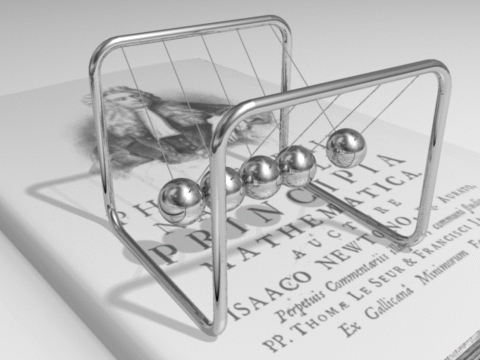
\includegraphics[width=0.44\textwidth]{Newtons_cradle_animation_book}
% % \end{wrapfigure}
% \end{image}
% \captionof{figure}{Een fascinerend speeltje} 
	
De derde bewegingswet van Newton -- ook wel de wet van actie en reactie genoemd -- geeft de relatie tussen de krachten die lichamen onderling op elkaar uitoefenen.

\begin{definition}[De wet van actie en reactie]\nl

Wanneer lichaam A op lichaam B een kracht uitoefent, oefent lichaam B op lichaam A een even grote maar tegengestelde kracht uit. In symbolen:
\begin{equation*}
	\vec{F}_{a,b}=-\vec{F}_{b,a}
\end{equation*}
\end{definition}

\begin{expandable}{remark}{De actie- en reactiekracht zijn altijd even groot.}
	Het even groot zijn van die krachten is misschien opmerkelijk. Het is toch de appel die naar de aarde valt en niet andersom?! Of, als de kracht die de aarde op de appel uitoefent even groot is als die de appel op de aarde uitoefent, waarom gaan ze dan niet naar mekaar toe? Het antwoord is dat de \emph{uitwerking} van een kracht niet hetzelfde is als de kracht zelf. De massa van de aarde is gigantisch veel groter dan die van de appel zodat die, volgens de tweede wet van Newton, een veel kleinere versnelling krijgt. En het is de versnelling die we zien, niet de kracht.
\end{expandable}

\begin{expandable}{remark}{Van het krachtenpaar grijpen de krachten op verschillende lichamen aan.}
	Er is altijd een voorwerp \emph{waardoor} de kracht wordt uitgeoefend en een voorwerp \emph{waarop} de kracht wordt uitgeoefend.

	\begin{denkvraag*}{}%{Boer Teun en zijn ezel Donkey}
		De ezel van boer Teun, Donkey, wil de kar met waar voor de markt niet trekken. Hij maakt namelijk de volgende redenering: `Voor elke poging die ik doe om de wagen vooruit te trekken, oefent de kar een even grote maar achterwaartse kracht uit. De nettokracht zal dan ook onvermijdelijk altijd nul zijn, zodat ik niet in beweging zal geraken. Ik doe geen moeite.'

		Waar loopt de redenering van de ezel mis?
	\end{denkvraag*}

\end{expandable}

\begin{expandable}{remark}{Actie- en reactiekracht zijn niet eenduidig.}
	Omdat de twee krachten van het krachtenpaar tegelijk optreden, is het in feite niet mogelijk aan te geven wie nu de actiekracht en wie de reactiekracht is.
\end{expandable}

Met deze derde wet kunnen we verschillende verschijnselen verklaren. Hier volgen enkele voorbeelden.

\begin{example}[Hoe kunnen we eigenlijk lopen?] \nl
	Zo is de wet van actie en reactie van toepassing op wandelen. Wij kunnen vanuit rust in beweging komen door ons af te zetten. Wij oefenen een kracht op de grond uit waarbij deze laatste op zijn beurt een even grote en tegengestelde kracht op ons uitoefent. Zo krijgen wij een versnelling. 

\end{example}

\begin{example}[Hoe stuwt een raket zich voort?]\nl
	Een vliegtuig met straalmotoren of een raket doen hetzelfde. Door het uitoefenen van een kracht op de naar achter uitgeworpen gassen, oefenen de uitgeworpen gassen een kracht uit op het vliegtuig of de raket. Maar dan voorwaarts. (Een vliegtuig of raket duwt zich dus niet af tegen de (eventuele) lucht.)
\end{example}

\begin{exercise}
	Een grote magneet oefent op een ijzeren spijkertje een kracht uit. Welke van de volgende uitspraken is dan juist?
	\begin{multipleChoice}
		\choice{Het spijkertje zelf oefent op de magneet geen kracht uit.}
		\choice{De kracht die het spijkertje op de magneet uitoefent is veel kleiner dan deze door de magneet op het spijkertje uitgeoefend.}
		\choice[correct]{De kracht die het spijkertje op de magneet uitoefent is even groot als deze door de magneet op het spijkertje uitgeoefend.}
		\choice{Over de grootte van de kracht die het spijkertje op de magneet uitoefent, kan niets met zekerheid gezegd worden.}
	\end{multipleChoice}
	% \begin{oplossing}
	% 	c
	% 	% $\answer[onlineshowanswerbutton]{(c)}$
	% \end{oplossing}
\end{exercise}

\begin{exercise}
	Je springt vanuit een roeibootje naar de oever. Verklaar wat er kan gebeuren als het roeibootje niet of wel vastgemeerd is. Wanneer je nu vanaf een groot binnenschip naar de oever springt, wat zou het resultaat dan zijn? Verklaar!
	\begin{oplossing}
		Bij een roeibootje dat niet vastgemeerd is, is er veel kans dat je in het water belandt. Bij het afzetten, schiet het bootje namelijk gemakkelijk onder je weg. Hoe komt dat? Wel, doordat je je afzet, oefen je een kracht uit op het bootje. De \textbf{derde wet van Newton} zegt dat het bootje dan een even grote kracht op jou uitoefent, in de tegengestelde richting. Het is die reactiekracht die je zou willen aanwenden om op de oever te geraken. De massa van het bootje is echter zo klein in vergelijking met jouw massa dat, volgens de \textbf{tweede wet van Newton} ($\vec{F}=m\vec{a}$), de versnelling die het bootje krijgt als gevolg van jouw actiekracht veel groter is dan de versnelling die je zelf krijgt door de afzet. In de korte tijd dat je jezelf kan afzetten, verwerft het bootje dus een grote snelheid waardoor het onder je wegschiet en krijg jij geen noemenswaardige snelheid opgebouwd.

		Als het bootje is vastgemeerd, lukt het je wel de oever te bereiken. Het bootje kan immers niet wegschieten waardoor je je voldoende lang kan afzetten (er werkt voldoende lang een kracht op jou) en zo de nodige snelheid kan verwerven (je krijgt immers een versnelling) om de sprong te kunnen maken.

		Voor een groot binnenschip is de massa zo groot in vergelijking met die van jou, dat het binnenschip een verwaarloosbare versnelling weg van de oever krijgt. Je kan een voldoende grote versnelling opbouwen die lang genoeg aanhoudt om je op de oever te krijgen.
	\end{oplossing}
\end{exercise}

\begin{exercise}
	Twee ploegen zijn aan het touwtrekken. Volgens het derde beginsel van Newton oefenen de twee ploegen steeds even grote maar tegengestelde krachten op elkaar uit. Hoe is het dan mogelijk dat er toch een winnende ploeg is?
	\begin{oplossing}
		Er is een winnende ploeg mogelijk omdat het samenstellen van krachten op elke ploeg afzonderlijk gebeurt. Het zijn niet de actie- en reactiekracht (derde wet van Newton) die worden samengesteld. 
		
		De winnende ploeg slaagt erin zich beter af te zetten dan de verliezende ploeg. Dat wil zeggen dat de reactiekracht van de kracht die ze op de grond uitoefenen (de weerstandskracht dus) groter is dan de kracht tussen de twee ploegen. De resulterende kracht van de weerstandskracht en de spankracht op de ploeg, zorgt volgens de tweede wet van Newton voor een versnelling; de ploeg komt in beweging. Voor de verliezende groep is dat net omgekeerd.
	\end{oplossing}
\end{exercise}

\begin{exercise}
	Een eekhoorntje glijdt over een gladde tafel met een heleboel nootjes tussen zijn voorpoten. Wat zou het moeten doen om te verhinderen dat het van de tafel valt? Leg uit.
	
	\begin{oplossing}
		Het eekhoorntje moet de noten \emph{voor} zich uit gooien. De reactiekracht van de kracht die de eekhoorn op de nootjes uitoefent, grijpt aan op de eekhoorn en is tegengesteld gericht. Die reactiekracht kan hem afremmen en hem verhinderen van de tafel te glijden.
	\end{oplossing}
\end{exercise}

\end{document}

% Te verwerken?


% Om over na te denken: hoe kan een star lichaam een kracht uitoefenen?

% \begin{remark}\nl
% 	tegengesteld
% \end{remark}

% \begin{remark}\nl
% 	op elk moment, zonder vertraging
% \end{remark}
